\documentclass{article}
\usepackage[a4paper]{geometry}
% \usepackage[]{xlop}
\usepackage[]{amsmath}
\usepackage{url}
\usepackage[]{graphicx}
\usepackage{algorithm}
\usepackage{algpseudocode}
\usepackage[utf8]{inputenc}

\title{Fast Multiplication using Vedic Math}
\author{Soumye Singhal}
\date{6 March 2017}

\begin{document}

\maketitle
\tableofcontents
\newpage

\section{Introduction}
Traditional long mulitplication method \cite{google} takes a lot of time and are also generally difficult to carry out accurately and fastly in the head. For more details on the long division method go to : \url{http://mathworld.wolfram.com/LongMultiplication.html}. There are various methods given in vedas to multiply some specific type of 2-digit numbers very quickly. Two such examples are listed below. \cite{vedas} \cite{vedic}

\begin{table}[h]
	\begin{center}
		\begin{tabular}{|r | l|}
			\hline
			\textbf{TYPE} & \textbf{DESCRIPTION} \\
			\hline
			Type I & Two digit numbers with first digit same, and the last ones add up to 10. \\
			\hline
			Type II & Two digit numbers with first digit add up to 10, and the last ones are same. \\
			\hline
		\end{tabular}
		\caption{Table of Types}
	\end{center}
\end{table}

\section{Type I}
\subsection{Algorithm}
\label{Type I:algorithm}
	\begin{algorithm}
		\begin{algorithmic}
			\Procedure{Multiplication}{$a, b$}
				\State $c \gets a/10$ \Comment{First digit of the first number}	
				\State $d \gets a \; mod \; 10$ \Comment{Second digit of the first number}	
				\State $e \gets b/10$ \Comment{First digit of the second number}
				\State $f \gets b \; mod \; 10$ \Comment{Second digit of the second number}	
				\If{$c == e$ \& $d+f = 10$}
					\State $Part1 \gets c \times (c+1)$
					\State $Part2 \gets d \times f$
					\State $Product \gets Part1 \times 100 + Part2$ \Comment{Combining the two products}
					\State{\Return{$Product$}}
				\Else
					\State{\Return{Not of Type I}}
				\EndIf
			\EndProcedure
		\end{algorithmic}
	\end{algorithm}

\subsection{MindMap for Mental Calculation}
Using the algorithm given in \ref{Type I:algorithm} we can carry out this method in our mind in a way similar to the mindmap given in \ref{Figure1}
\newpage
\begin{figure}[h]
	\label{Figure1}
	\centering
	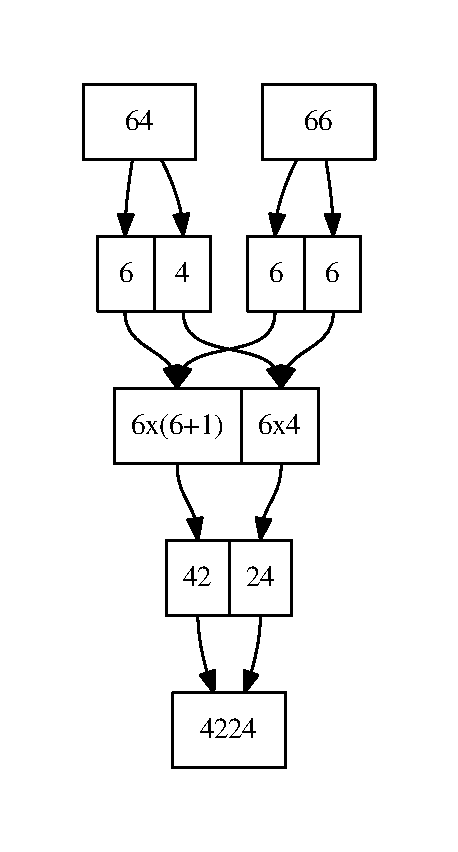
\includegraphics[scale=1]{g1.pdf} \\
	\caption{Type I}
\end{figure}
\newpage
\subsection{Algebraic Explanation}
We now give an algebraic explanation as to why the above stated algorithm works. Consider these two digit numbers as $ab$ and $a(10-b)$. Note that the first common digit is a and the second digits are b and 10-b respectively.
\begin{align*}
    ab  \times  a(10-b) & = ( 10a + b )( 10a + 10 - b ) \\
                 & = 100a^2 + 100a -10a \times b + 10a \times b + 10 \times b - b^2 \\
                 & = 100a \times (a+1) + b \times (10-b) \\
                 & = a \times (a+1) \; | \; b \times (10-b) \\
\end{align*}

\subsection{Extension}
For general case we can assume the product of two n digit numbers whose first k digits are same such that $k < n$ and the rest of n-k digit is such that the sum for both numbers in $ {10}^{n-k} $. Then again the product will be the concatenation of product of number formed by first k digits and its successor and product of number formed by rest of the digit and its subtraction from $ {10}^{n-k} $
\url {http://www.vedantatree.com/2012/05/vedic-math-multiplication-of-numbers.html}

\section{Type II}
\subsection{Algorithm}
\label{type II:algorithm}
	\begin{algorithm}
		\begin{algorithmic}
			\Procedure{Multiplication}{$a, b$}
				\State $c \gets a/10$ \Comment{First digit of the first number}	
				\State $d \gets a \; \mod \; 10$ \Comment{Second digit of the first number}	
				\State $e \gets b/10$ \Comment{First digit of the second number}
				\State $f \gets b \; \mod \; 10$ \Comment{Second digit of the second number}	
				\If{$d = f$ \& $c+e = 10$}
					\State $Part1 \gets c \times e + d$
					\State $Part2 \gets d \times f$
					\State $Product \gets Part1 \times 100 + Part2$ \Comment{Combining the two products}
					\State{\Return{$Product$}}
				\Else
					\State{\Return{Not of Type II}}
				\EndIf
			\EndProcedure
		\end{algorithmic}
	\end{algorithm}


\subsection{MindMap for Mental Calculation}
Using the algorithm given in \ref{type II:algorithm} we can carry out this method in our mind in a way similar to the mindmap given in \ref{Figure2}
\footnote{Note: Here we assume that the person is comfortable with 1 digit multipliction.}
\newpage
\begin{figure}[h]
	\label{Figure2}
	\centering
	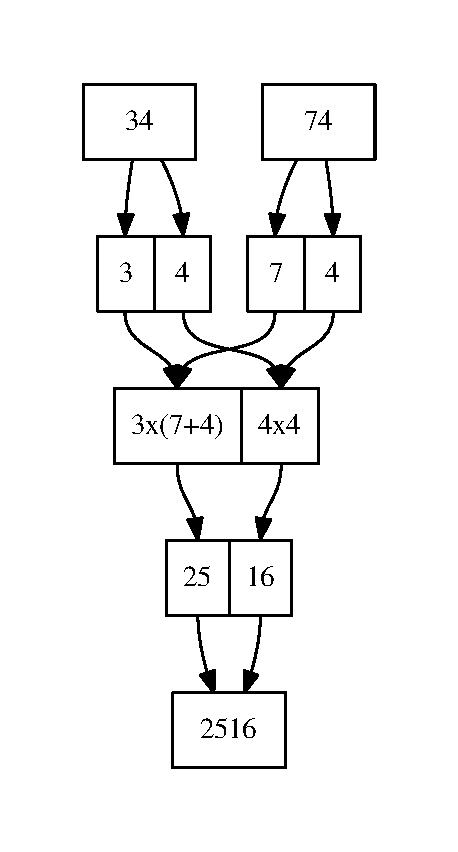
\includegraphics[scale=1]{g2.pdf} \\
	\caption{Type II}
\end{figure}
\newpage
\subsection{Algebraic Explanation}
We now give an algebraic explanation as to why the above stated algorithm works. Consider these two digit numbers as $ab$ and $(10-a)b$. Note that the second common digit is b and the first digits are a and 10-a respectively.
\begin{align*}
    ab  \times  (10-a)b & = ( 10a + b )( 10(10 - a) + b ) \\
                 & = ( 10a + b )( 100 - 10a + b ) \\
                 & = 1000a - 100a^2 + 10a \times b + 100b - 10a \times b + b^2 \\
                 & = 100(10a - a^2 + b) + b^2 \\
                 & = 100(a(10 - a) + b) + b^2 \\
                 & = a(10 - a) + b \; | \; b^2 \\   
\end{align*}
\subsection{Extension}
For general case we can assume the product of two n digit numbers whose last k digits are same such that $k < n$ and the rest of n-k digit is such that the sum for both numbers in $ {10}^{n-k} $. Then again the product will be the concatenation of product of number formed by first k digits added with the last k digits and the square of number formed by rest of the digit.
\url {http://www.vedantatree.com/2012/05/vedic-math-multiplication-of-numbers.html}

\section{Why these Methods are Faster}
In regular multiplication of two 2-digit numbers we need to do 4 1-1 digit multiplications. But in this shorter method we need to only do 2 1-1 digit multiplications and 2 simple additions. This makes it less time consuming and efficient. Also since it takes only a short part of the working memory, so one is able to do it easily.


\bibliographystyle{abbrv}
\bibliography{bibl}
\end{document}
